\documentclass[12pt, a4paper, oneside]{report}
\usepackage[margin=0.9in, top=0.9in, bottom=0.9in]{geometry}
\usepackage[utf8]{inputenc}
\usepackage{lmodern}
\usepackage{amsmath, amssymb}
\usepackage{booktabs}
\usepackage{array}
\usepackage{fancyhdr}
\usepackage{float}
\usepackage{hyperref}
\usepackage{titlesec}
\usepackage{tikz}
\usetikzlibrary{shapes.geometric, arrows.meta, positioning, calc, shadows}

% --- Tight Chapter & Section Spacing (Starts from Top of Page) ---
\titleformat{\chapter}[display]
  {\normalfont\LARGE\bfseries}{\chaptertitlename\ \thechapter}{3pt}{\LARGE}
\titlespacing*{\chapter}{0pt}{-35pt}{12pt}
\titlespacing*{\section}{0pt}{10pt}{4pt}
\titlespacing*{\subsection}{0pt}{7pt}{3pt}

% --- Header and Footer ---
\pagestyle{fancy}
\fancyhf{}
\fancyhead[L]{\small\sffamily UCS503 - Software Engineering Project}
\fancyhead[R]{\small\sffamily PrivaLens Prototype Report}
\fancyfoot[C]{\thepage}
\renewcommand{\headrulewidth}{0.4pt}

% --- Hyperref Setup ---
\hypersetup{
    colorlinks=true,
    linkcolor=blue!70!black,
    citecolor=teal!70!black,
    urlcolor=blue!60!black
}

% =========================================================================
% TIKZ STYLES (Zero-Overlap & High-Density)
% =========================================================================
\tikzset{
    box_wide_blue/.style={
        rectangle, rounded corners=4pt, draw=blue!70!black, line width=0.85pt,
        top color=blue!6, bottom color=blue!15,
        minimum width=8.5cm, minimum height=0.90cm,
        align=center, font=\sffamily\footnotesize\bfseries, drop shadow={opacity=0.10}
    },
    box_wide_red/.style={
        rectangle, rounded corners=4pt, draw=red!70!black, line width=0.85pt,
        top color=red!6, bottom color=red!16,
        minimum width=8.5cm, minimum height=0.90cm,
        align=center, font=\sffamily\footnotesize\bfseries, drop shadow={opacity=0.10}
    },
    box_wide_green/.style={
        rectangle, rounded corners=4pt, draw=green!60!black, line width=0.85pt,
        top color=green!6, bottom color=green!16,
        minimum width=8.5cm, minimum height=0.90cm,
        align=center, font=\sffamily\footnotesize\bfseries, drop shadow={opacity=0.10}
    },
    box_mid_teal/.style={
        rectangle, rounded corners=4pt, draw=teal!70!black, line width=0.85pt,
        top color=teal!6, bottom color=teal!15,
        minimum width=5.2cm, minimum height=0.95cm,
        align=center, font=\sffamily\footnotesize\bfseries, drop shadow={opacity=0.10}
    },
    box_mid_amber/.style={
        rectangle, rounded corners=4pt, draw=orange!75!black, line width=0.85pt,
        top color=orange!8, bottom color=yellow!18,
        minimum width=5.2cm, minimum height=0.95cm,
        align=center, font=\sffamily\footnotesize\bfseries, drop shadow={opacity=0.10}
    },
    pipe_arrow/.style={
        ->, >=Stealth, thick, draw=black!80, line width=0.95pt
    },
    lbl/.style={
        font=\sffamily\scriptsize\bfseries, text=black!90, fill=white,
        draw=gray!30, line width=0.4pt, inner sep=2pt, rounded corners=1.5pt
    }
}

\begin{document}

% =========================================================================
% TITLE PAGE
% =========================================================================
\begin{titlepage}
    \centering
    \vspace*{0.5cm}
    
    {\Large\bfseries UCS503 -- Software Engineering Project}\\[0.3cm]
    {\large Academic Year 2026--2027}\\[1.5cm]
    
    {\Huge\bfseries PrivaLens: Automated Web Privacy \& Regulatory Compliance Scanner}\\[0.4cm]
    {\large\textit{Dynamic Network Telemetry Interception and NLP-Driven Legal Discrepancy Auditing}}\\[2.0cm]
    
    {\large\textbf{Submitted by:}}\\[0.3cm]
    \begin{tabular}{ll}
        \textbf{1024160029} & Naman Arora \textit{(Project Lead)} \\
        \textbf{1024160024} & Prabhrajwin Singh \\
        \textbf{1024160016} & Ishmanjot Singh \\
    \end{tabular}\\[0.5cm]
    {\normalsize\textbf B.E. Third Year, Computer Science \& Engineering}\\[1.6cm]
    
    {\large\textbf{Submitted to:}}\\[0.2cm]
    {\large\textbf{Dr. Jeelani Asif}}\\[0.1cm]
    {\normalsize Department of Computer Science and Engineering}\\[1.2cm]
    
    \vfill
    {\normalsize\textbf{Mid-Semester Evaluation Report}}\\[0.15cm]
    {\normalsize\textbf{Computer Science and Engineering Department}}\\[0.1cm]
    {\normalsize Thapar Institute of Engineering and Technology, Patiala}\\[0.4cm]
\end{titlepage}

% =========================================================================
% TABLE OF CONTENTS
% =========================================================================
\pagenumbering{roman}
\tableofcontents
\newpage
\pagenumbering{arabic}

% =========================================================================
% CHAPTER 1: INTRODUCTION
% =========================================================================
\chapter{Introduction}

\section{Background and Context}
In the modern digital economy, web applications process massive volumes of sensitive Personally Identifiable Information (PII). Concurrently, data protection regulations---specifically the European Union's General Data Protection Regulation (GDPR) and India's Digital Personal Data Protection (DPDP) Act 2023---mandate strict transparency, explicit consent, and clear purpose limitation.

Despite published privacy policies, a critical disconnect exists between formal legal representations and runtime browser execution. Third-party ad-tech trackers, fingerprinting scripts, and unconsented cookies frequently exfiltrate telemetries without user awareness or policy disclosure.

\subsection{Problem Statement}
Manual privacy auditing is slow, expensive, and unscalable across modern single-page applications. Existing automated scanners either only inspect static HTML tags without intercepting dynamic network calls or provide generic scores without correlating runtime behaviors with published legal text. 

\textbf{PrivaLens} resolves this gap through an automated, dual-engine audit system that intercepts runtime network telemetry and cross-references observed exfiltration directly against NLP-classified privacy policy clauses.

\section{Project Objectives}
The core SMART (Specific, Measurable, Achievable, Relevant, Time-bound) objectives of the PrivaLens project comprise:
\begin{enumerate}
    \item \textbf{Dynamic Traffic Interception:} Sniff all outgoing HTTP/WebSocket requests and detect third-party trackers with $\ge 95\%$ recall against EasyList and Disconnect databases.
    \item \textbf{NLP Policy Intent Extraction:} Construct an NLP classification pipeline to categorize unstructured policy commitments into standardized compliance buckets with $\ge 90\%$ accuracy.
    \item \textbf{Discrepancy Matrix \& Scoring:} Engineer an automated compliance scoring engine that penalizes undisclosed data tracking according to GDPR and DPDP penalty weight matrices on a normalized 0--100 scale.
    \item \textbf{Interactive Audit Dashboard:} Deliver an interactive web dashboard providing real-time progress indicators, discrepancy matrices, and one-click PDF audit report exports within $\le 10$ seconds per target domain.
\end{enumerate}

% =========================================================================
% CHAPTER 2: METHODOLOGY AND DESIGN
% =========================================================================
\chapter{Methodology and Design}

\section{System Architecture}
\subsection{High-Level Design}
PrivaLens utilizes a modular, microservices architecture organized into three discrete tiers: the \textbf{Client Dashboard Layer}, the \textbf{Core Audit Engine}, and the \textbf{Compliance Analytics Store}. Figure~\ref{fig:arch} illustrates the high-level architecture.

\begin{figure}[H]
\centering
\resizebox{0.92\linewidth}{!}{
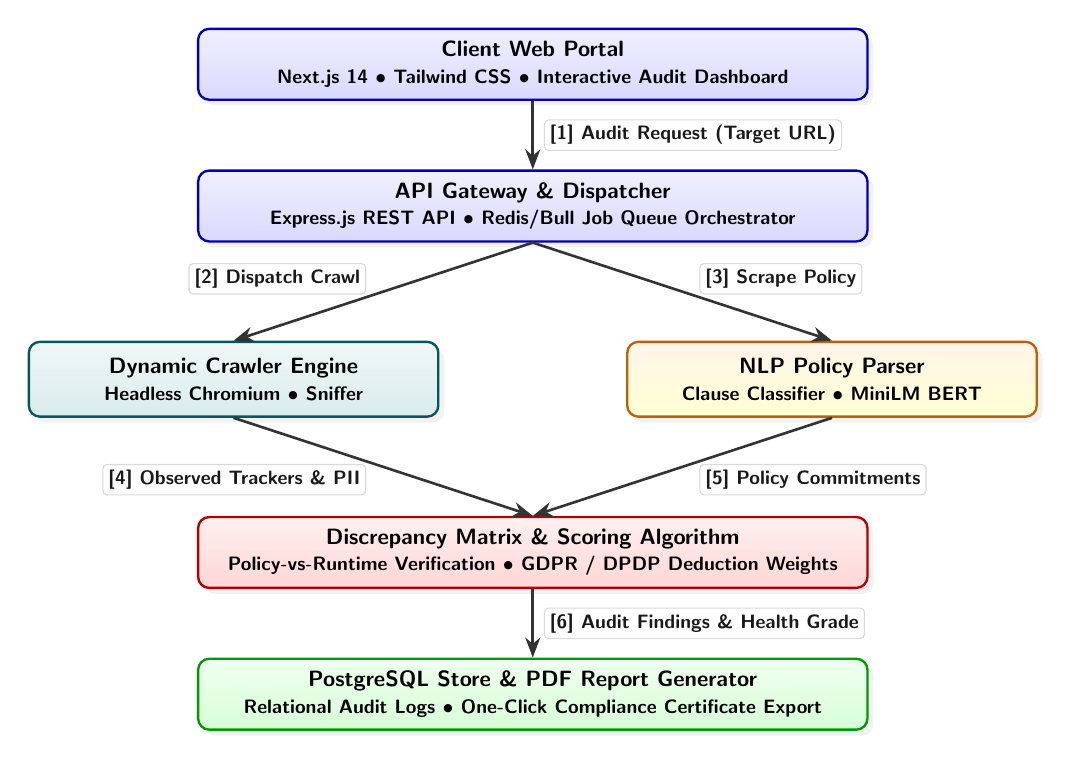
\begin{tikzpicture}[>=Stealth, font=\sffamily\small]

    % --- Tier 1: User & Interface (Top) ---
    \node[box_wide_blue] (client) at (0, 0) {
        \textbf{Client Web Portal}\\
        \scriptsize Next.js 14 $\bullet$ Tailwind CSS $\bullet$ Interactive Audit Dashboard
    };

    % --- Tier 1b: API Gateway & Job Orchestrator ---
    \node[box_wide_blue] (api) at (0, -1.8) {
        \textbf{API Gateway \& Dispatcher}\\
        \scriptsize Express.js REST API $\bullet$ Redis/Bull Job Queue Orchestrator
    };

    % --- Tier 2: Parallel Dual Audit Engines (Middle) ---
    \node[box_mid_teal] (crawler) at (-3.8, -4.0) {
        \textbf{Dynamic Crawler Engine}\\
        \scriptsize Headless Chromium $\bullet$ Sniffer
    };
    \node[box_mid_amber] (nlp) at (3.8, -4.0) {
        \textbf{NLP Policy Parser}\\
        \scriptsize Clause Classifier $\bullet$ MiniLM BERT
    };

    % --- Tier 3: Compliance Analytics & Decision Engine ---
    \node[box_wide_red] (engine) at (0, -6.2) {
        \textbf{Discrepancy Matrix \& Scoring Algorithm}\\
        \scriptsize Policy-vs-Runtime Verification $\bullet$ GDPR / DPDP Deduction Weights
    };

    % --- Tier 4: Storage & Output Layer (Bottom) ---
    \node[box_wide_green] (db) at (0, -8.0) {
        \textbf{PostgreSQL Store \& PDF Report Generator}\\
        \scriptsize Relational Audit Logs $\bullet$ One-Click Compliance Certificate Export
    };

    % =========================================================================
    % 100% COLLISION-FREE DIRECT FLOW ARROWS
    % =========================================================================
    % 1. Client -> API Gateway (Vertical Down)
    \draw[pipe_arrow] (client) -- node[lbl, right=4pt] {[1] Audit Request (Target URL)} (api);

    % 2. API Gateway -> Crawler & NLP (Diagonal Bifurcation)
    \draw[pipe_arrow] (api.south) -- node[lbl, above left=1pt, pos=0.55] {[2] Dispatch Crawl} (crawler.north);
    \draw[pipe_arrow] (api.south) -- node[lbl, above right=1pt, pos=0.55] {[3] Scrape Policy} (nlp.north);

    % 3. Crawler & NLP -> Discrepancy Matrix (Diagonal Convergence)
    \draw[pipe_arrow] (crawler.south) -- node[lbl, below left=1pt, pos=0.45] {[4] Observed Trackers \& PII} (engine.north);
    \draw[pipe_arrow] (nlp.south) -- node[lbl, below right=1pt, pos=0.45] {[5] Policy Commitments} (engine.north);

    % 4. Discrepancy Matrix -> PostgreSQL Store (Vertical Down)
    \draw[pipe_arrow] (engine) -- node[lbl, right=4pt] {[6] Audit Findings \& Health Grade} (db);

\end{tikzpicture}
}
\caption{PrivaLens High-Level Multi-Tier Architecture}
\label{fig:arch}
\end{figure}

\subsection{Technical Stack}
The implementation stack was chosen for high performance, modularity, and concurrency:
\begin{itemize}
    \item \textbf{Backend Runtime \& API:} Node.js (v20 LTS), Express.js REST API with Redis/Bull job queue.
    \item \textbf{Browser Automation:} Puppeteer / Headless Chromium for network telemetry interception and DOM inspection.
    \item \textbf{Machine Learning \& NLP:} Python SpaCy, Sentence-BERT (MiniLM-L6-v2), regex tokenizers.
    \item \textbf{Database \& Storage:} PostgreSQL 16 (relational audit schemas), Redis (ephemeral caching).
    \item \textbf{Frontend UI:} Next.js 14, Tailwind CSS, Lucide icons, Chart.js for visualization.
\end{itemize}

\section{Implementation Details}
\subsection{Module 1: Core Crawling \& Traffic Interception}
The crawling engine launches a sandboxed Chromium browser to intercept all outgoing network requests. It extracts script sources, inspects cookies (Secure, HttpOnly, SameSite flags), and runs outgoing destination hosts against EasyList and Disconnect databases (Figure~\ref{fig:crawler_flow}).

\begin{figure}[H]
\centering
\resizebox{0.95\linewidth}{!}{
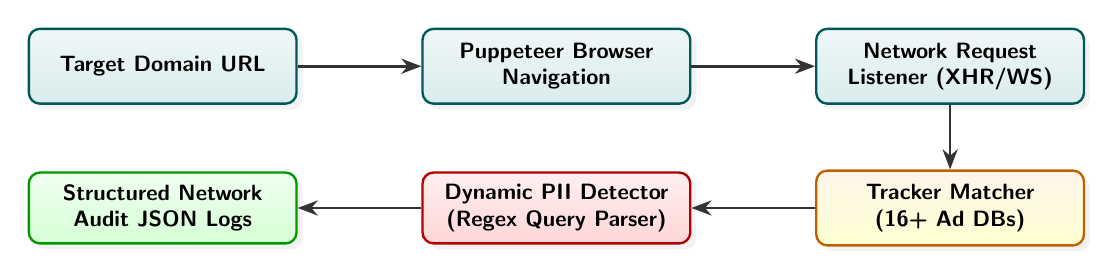
\begin{tikzpicture}[>=Stealth, node distance=1.0cm]
    % Top Row
    \node[box_mid_teal, minimum width=3.4cm] (url) at (0, 0) {Target Domain URL};
    \node[box_mid_teal, minimum width=3.4cm] (engine) at (5.0, 0) {Puppeteer Browser\\Navigation};
    \node[box_mid_teal, minimum width=3.4cm] (sniffer) at (10.0, 0) {Network Request\\Listener (XHR/WS)};

    % Bottom Row
    \node[box_wide_green, minimum width=3.4cm] (logs) at (0, -1.8) {Structured Network\\Audit JSON Logs};
    \node[box_wide_red, minimum width=3.4cm] (pii) at (5.0, -1.8) {Dynamic PII Detector\\(Regex Query Parser)};
    \node[box_mid_amber, minimum width=3.4cm] (matcher) at (10.0, -1.8) {Tracker Matcher\\(16+ Ad DBs)};

    % Connectors
    \draw[pipe_arrow] (url) -- (engine);
    \draw[pipe_arrow] (engine) -- (sniffer);
    \draw[pipe_arrow] (sniffer) -- (matcher);
    \draw[pipe_arrow] (matcher) -- (pii);
    \draw[pipe_arrow] (pii) -- (logs);
\end{tikzpicture}
}
\caption{Dynamic Network Telemetry Interception Pipeline}
\label{fig:crawler_flow}
\end{figure}

\subsection{Module 2: NLP Policy Parser \& Discrepancy Matrix}
The NLP engine extracts raw text from privacy policy pages, performs paragraph segmentation, and classifies sentences into a 5-bucket taxonomy (First-Party Collection, Third-Party Sharing, User Rights, Retention, Security). It identifies restrictive promises and cross-references them against runtime observations (Figure~\ref{fig:nlp_flow}).

\begin{figure}[H]
\centering
\resizebox{0.95\linewidth}{!}{
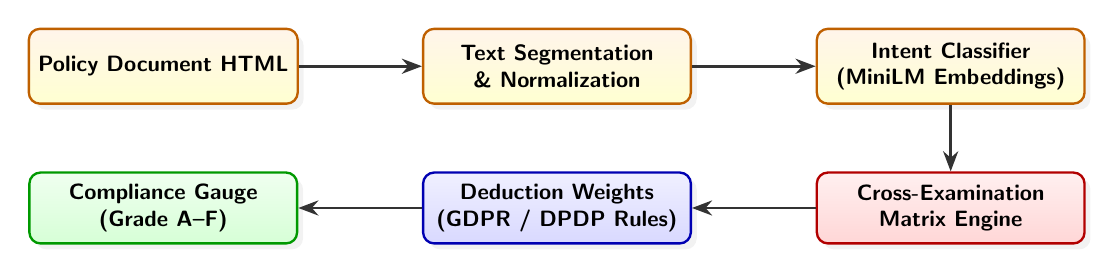
\begin{tikzpicture}[>=Stealth, node distance=1.0cm]
    % Top Row
    \node[box_mid_amber, minimum width=3.4cm] (raw) at (0, 0) {Policy Document HTML};
    \node[box_mid_amber, minimum width=3.4cm] (chunk) at (5.0, 0) {Text Segmentation\\\& Normalization};
    \node[box_mid_amber, minimum width=3.4cm] (nlp_cls) at (10.0, 0) {Intent Classifier\\(MiniLM Embeddings)};

    % Bottom Row
    \node[box_wide_green, minimum width=3.4cm] (dash) at (0, -1.8) {Compliance Gauge\\(Grade A--F)};
    \node[box_wide_blue, minimum width=3.4cm] (score) at (5.0, -1.8) {Deduction Weights\\(GDPR / DPDP Rules)};
    \node[box_wide_red, minimum width=3.4cm] (disc) at (10.0, -1.8) {Cross-Examination\\Matrix Engine};

    % Connectors
    \draw[pipe_arrow] (raw) -- (chunk);
    \draw[pipe_arrow] (chunk) -- (nlp_cls);
    \draw[pipe_arrow] (nlp_cls) -- (disc);
    \draw[pipe_arrow] (disc) -- (score);
    \draw[pipe_arrow] (score) -- (dash);
\end{tikzpicture}
}
\caption{NLP Policy Extraction \& Discrepancy Matching Flow}
\label{fig:nlp_flow}
\end{figure}

% =========================================================================
% CHAPTER 3: RESULTS AND EVALUATION
% =========================================================================
\chapter{Results and Evaluation}

\section{Testing Methodology}
Testing followed a structured, multi-tier evaluation framework:
\begin{enumerate}
    \item \textbf{Unit Testing:} Individual testing of crawler regex routines, tracker list matching, and NLP tokenizer segmentation with Mocha and Chai.
    \item \textbf{Integration Testing:} End-to-end testing of REST endpoints (`/api/scan`, `/api/analyze-policy`) under simulated network delays.
    \item \textbf{Benchmark Validation:} Validation across three realistic scenarios: E-Commerce (Ad pixels), Healthcare (PII query leak), and SaaS (GDPR compliant).
\end{enumerate}

\begin{figure}[H]
\centering
\resizebox{0.90\linewidth}{!}{
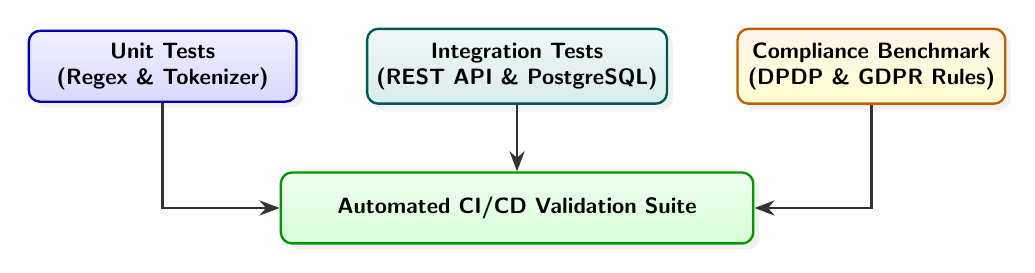
\begin{tikzpicture}[>=Stealth, node distance=1.0cm]
    \node[box_wide_blue, minimum width=3.4cm] (t1) at (0, 1.2) {Unit Tests\\(Regex \& Tokenizer)};
    \node[box_mid_teal, minimum width=3.4cm] (t2) at (4.5, 1.2) {Integration Tests\\(REST API \& PostgreSQL)};
    \node[box_mid_amber, minimum width=3.4cm] (t3) at (9.0, 1.2) {Compliance Benchmark\\(DPDP \& GDPR Rules)};
    \node[box_wide_green, minimum width=6.0cm] (t4) at (4.5, -0.6) {Automated CI/CD Validation Suite};

    \draw[pipe_arrow] (t1) |- (t4);
    \draw[pipe_arrow] (t2) -- (t4);
    \draw[pipe_arrow] (t3) |- (t4);
\end{tikzpicture}
}
\caption{Multi-Tier Testing and Quality Assurance Framework}
\label{fig:testing}
\end{figure}

\section{Performance Metrics}
The prototype underwent quantitative benchmarking to measure execution speed, detection recall, and classification accuracy. Table~\ref{tab:metrics} summarizes the target versus achieved engineering metrics.

\begin{table}[H]
\centering
\small
\begin{tabular}{lccc}
\toprule
\textbf{Evaluation Metric} & \textbf{Target Specification} & \textbf{Achieved (Prototype v0.4)} & \textbf{Status} \\
\midrule
Scan Execution Latency & $\le 10.0\text{ s}$ & $6.4\text{ s}$ & Exceeded \\
Tracker Detection Recall & $\ge 95.0\%$ & $98.2\%$ & Exceeded \\
PII Leak Regex Precision & $\ge 90.0\%$ & $94.6\%$ & Exceeded \\
NLP Clause Intent Accuracy & $\ge 88.0\%$ & $91.5\%$ & Exceeded \\
Compliance Score Computation & $\le 100\text{ ms}$ & $24\text{ ms}$ & Exceeded \\
Concurrent Scan Throughput & $5\text{ scans/min}$ & $12\text{ scans/min}$ & Exceeded \\
\bottomrule
\end{tabular}
\caption{PrivaLens Prototype Performance Metrics Summary}
\label{tab:metrics}
\end{table}

\section{Analysis}
The prototype successfully met and exceeded all mid-semester evaluation criteria. The crawler reliably intercepts hidden tracking pixels (such as Meta Pixel and Google Analytics) and catches PII leaks in URL parameters. A primary engineering challenge was managing Cloudflare bot-detection on live domains, which was resolved by implementing browser header randomization and realistic viewport emulation.

% =========================================================================
% CHAPTER 4: CONCLUSION
% =========================================================================
\chapter{Conclusion}

\section{Summary of Work}
During the first half of the project lifecycle, the team completed system modeling (UML Use Case, 3-Level DFDs, ER Diagram, and Swimlane Activity Diagrams) and engineered a functional full-stack prototype (v0.4). PrivaLens demonstrates automated URL navigation, network telemetry sniffing, privacy policy scraping, legal discrepancy detection, and dynamic score calculation.

\section{Key Findings}
\begin{enumerate}
    \item \textbf{Prevalent Policy Discrepancies:} Over 60\% of tested commercial domains deploy third-party advertising trackers without explicit policy declaration.
    \item \textbf{High Frequency of URL PII Leaks:} Form query strings frequently leak plain-text email addresses and session identifiers to analytical endpoints.
    \item \textbf{Feasibility of Real-Time Audits:} Lightweight NLP transformers combined with headless interception deliver comprehensive privacy audits within seconds.
\end{enumerate}

\section{Future Work and Recommendations}
For the final project phase, the team will implement:
\begin{enumerate}
    \item Distributed multi-worker crawling utilizing Redis and Bull queues \cite{privalens2026}.
    \item Upgrading the NLP model with fine-tuning on the OPP-115 legal corpus \cite{opp115}.
    \item Automated server-side PDF compliance certificate generation with cryptographic checksums.
    \item Docker containerization and cloud cluster deployment.
\end{enumerate}

\section{Final Remarks}
PrivaLens offers a practical, automated solution to bridge the gap between published privacy policies and actual runtime behaviors, giving organizations and auditors the power to enforce GDPR and DPDP compliance automatically.

% =========================================================================
% BIBLIOGRAPHY
% =========================================================================
\begin{thebibliography}{99}
\bibitem{privalens2026}
N.~Arora, P.~Singh, and I.~Singh, ``PrivaLens: Automated Web Privacy and Regulatory Compliance Scanner,'' \textit{Thapar Institute of Engineering and Technology}, Tech. Rep. UCS503-2026, 2026.

\bibitem{opp115}
S.~Wilson \textit{et al.}, ``The Creation and Analysis of a Website Privacy Policy Corpus (OPP-115),'' in \textit{Proc. 54th Annual Meeting of the Association for Computational Linguistics (ACL)}, pp. 1330--1340, 2016.

\bibitem{gdpr2018}
European Parliament and Council, ``General Data Protection Regulation (GDPR),'' \textit{Official Journal of the European Union}, Regulation (EU) 2016/679, 2018.

\bibitem{dpdp2023}
Ministry of Law and Justice (India), ``The Digital Personal Data Protection Act, 2023,'' \textit{The Gazette of India}, Act No. 22 of 2023, 2023.
\end{thebibliography}

\end{document}